\usetikzlibrary{positioning, shapes.geometric, arrows.meta, shadows, calc}

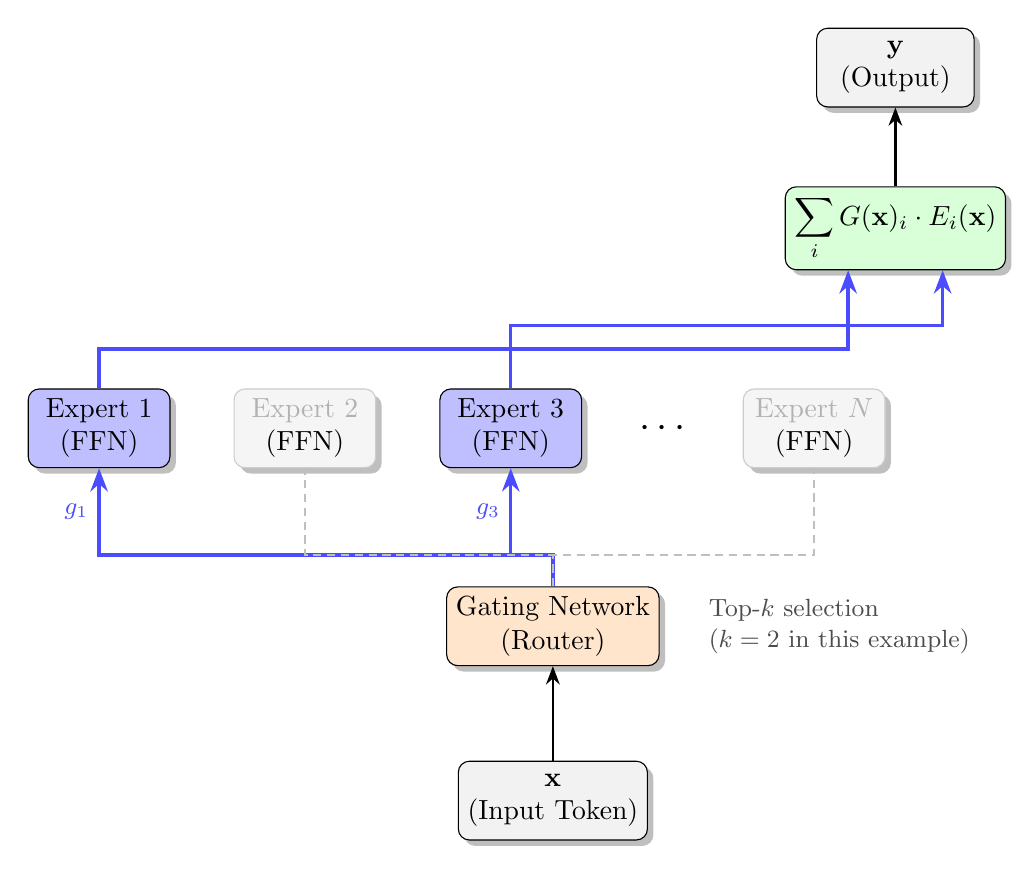
\begin{tikzpicture}[
    node distance=1cm and 1.2cm,
    block/.style={
        draw,
        rectangle,
        rounded corners,
        minimum width=2cm,
        minimum height=1cm,
        align=center,
        drop shadow
    },
    expert/.style={
        draw,
        rectangle,
        rounded corners,
        minimum width=1.8cm,
        minimum height=1cm,
        align=center,
        drop shadow
    },
    arrow/.style={
        ->,
        >=Stealth,
        thick
    },
    activearrow/.style={
        ->,
        >=Stealth,
        line width=1.2pt,
        blue!70
    },
    inactivearrow/.style={
        ->,
        >=Stealth,
        thick,
        densely dashed,
        draw=gray!50
    }
]

% Input
\node[block, fill=gray!10] (input) {$\mathbf{x}$\\(Input Token)};

% Router
\node[block, fill=orange!20, above=1.2cm of input] (router) {Gating Network\\(Router)};

% Experts row
\node[expert, fill=blue!25, above left=1.5cm and 3.5cm of router] (e1) {Expert 1\\(FFN)};
\node[expert, fill=gray!8, draw=gray!40, right=0.8cm of e1] (e2) {\color{gray!60}Expert 2\\(FFN)};
\node[expert, fill=blue!25, right=0.8cm of e2] (e3) {Expert 3\\(FFN)};
\node[right=0.6cm of e3, font=\Large] (dots) {$\cdots$};
\node[expert, fill=gray!8, draw=gray!40, right=0.6cm of dots] (en) {\color{gray!60}Expert $N$\\(FFN)};

% Weighted sum
\node[block, fill=green!15, above=1.5cm of router |- e1.north, xshift=4.35cm] (sum) {$\displaystyle\sum_{i} G(\mathbf{x})_i \cdot E_i(\mathbf{x})$};

% Output
\node[block, fill=gray!10, above=1cm of sum] (output) {$\mathbf{y}$\\(Output)};

% Input to Router
\draw[arrow] (input) -- (router);

% Router to active experts
\draw[activearrow] (router.north) -- ++(0, 0.4) -| (e1.south)
    node[pos=0.75, left, font=\small, text=blue!70] {$g_1$};
\draw[activearrow] (router.north) -- ++(0, 0.4) -| (e3.south)
    node[pos=0.75, left, font=\small, text=blue!70] {$g_3$};

% Router to inactive experts (dashed, no arrowhead)
\draw[densely dashed, gray!50, thick] (router.north) -- ++(0, 0.4) -| (e2.south);
\draw[densely dashed, gray!50, thick] (router.north) -- ++(0, 0.4) -| (en.south);

% Active experts to weighted sum
\draw[activearrow] (e1.north) -- ++(0, 0.5) -| ([xshift=-0.6cm]sum.south);
\draw[activearrow] (e3.north) -- ++(0, 0.8) -| ([xshift=0.6cm]sum.south);

% Weighted sum to output
\draw[arrow] (sum) -- (output);

% Annotations
\node[right=0.5cm of router, font=\small, text=black!70, align=left] (annot) {Top-$k$ selection\\($k = 2$ in this example)};


\end{tikzpicture}
